\section{Resultados}

\subsection{Segunda Consigna: Gráficos y Análisis}

\subsubsection{Red Doméstica}

Para la primera captura, se eligió una red domestica de uno de los integrantes del grupo.
La captura duro 30 minutos aproximados.
Al ser una red pequeña podemos distinguir fácilmente los nodos destacados.
La Figura~\ref{fig:red_domestica_network}. muestra 2 nodos destacados 192.168.0.1 que correspondes al router  y el nodo 192.168.0.27 correspondiente al PC desde donde se tomaron las capturas.

\begin{figure}[h!]
  \centering
   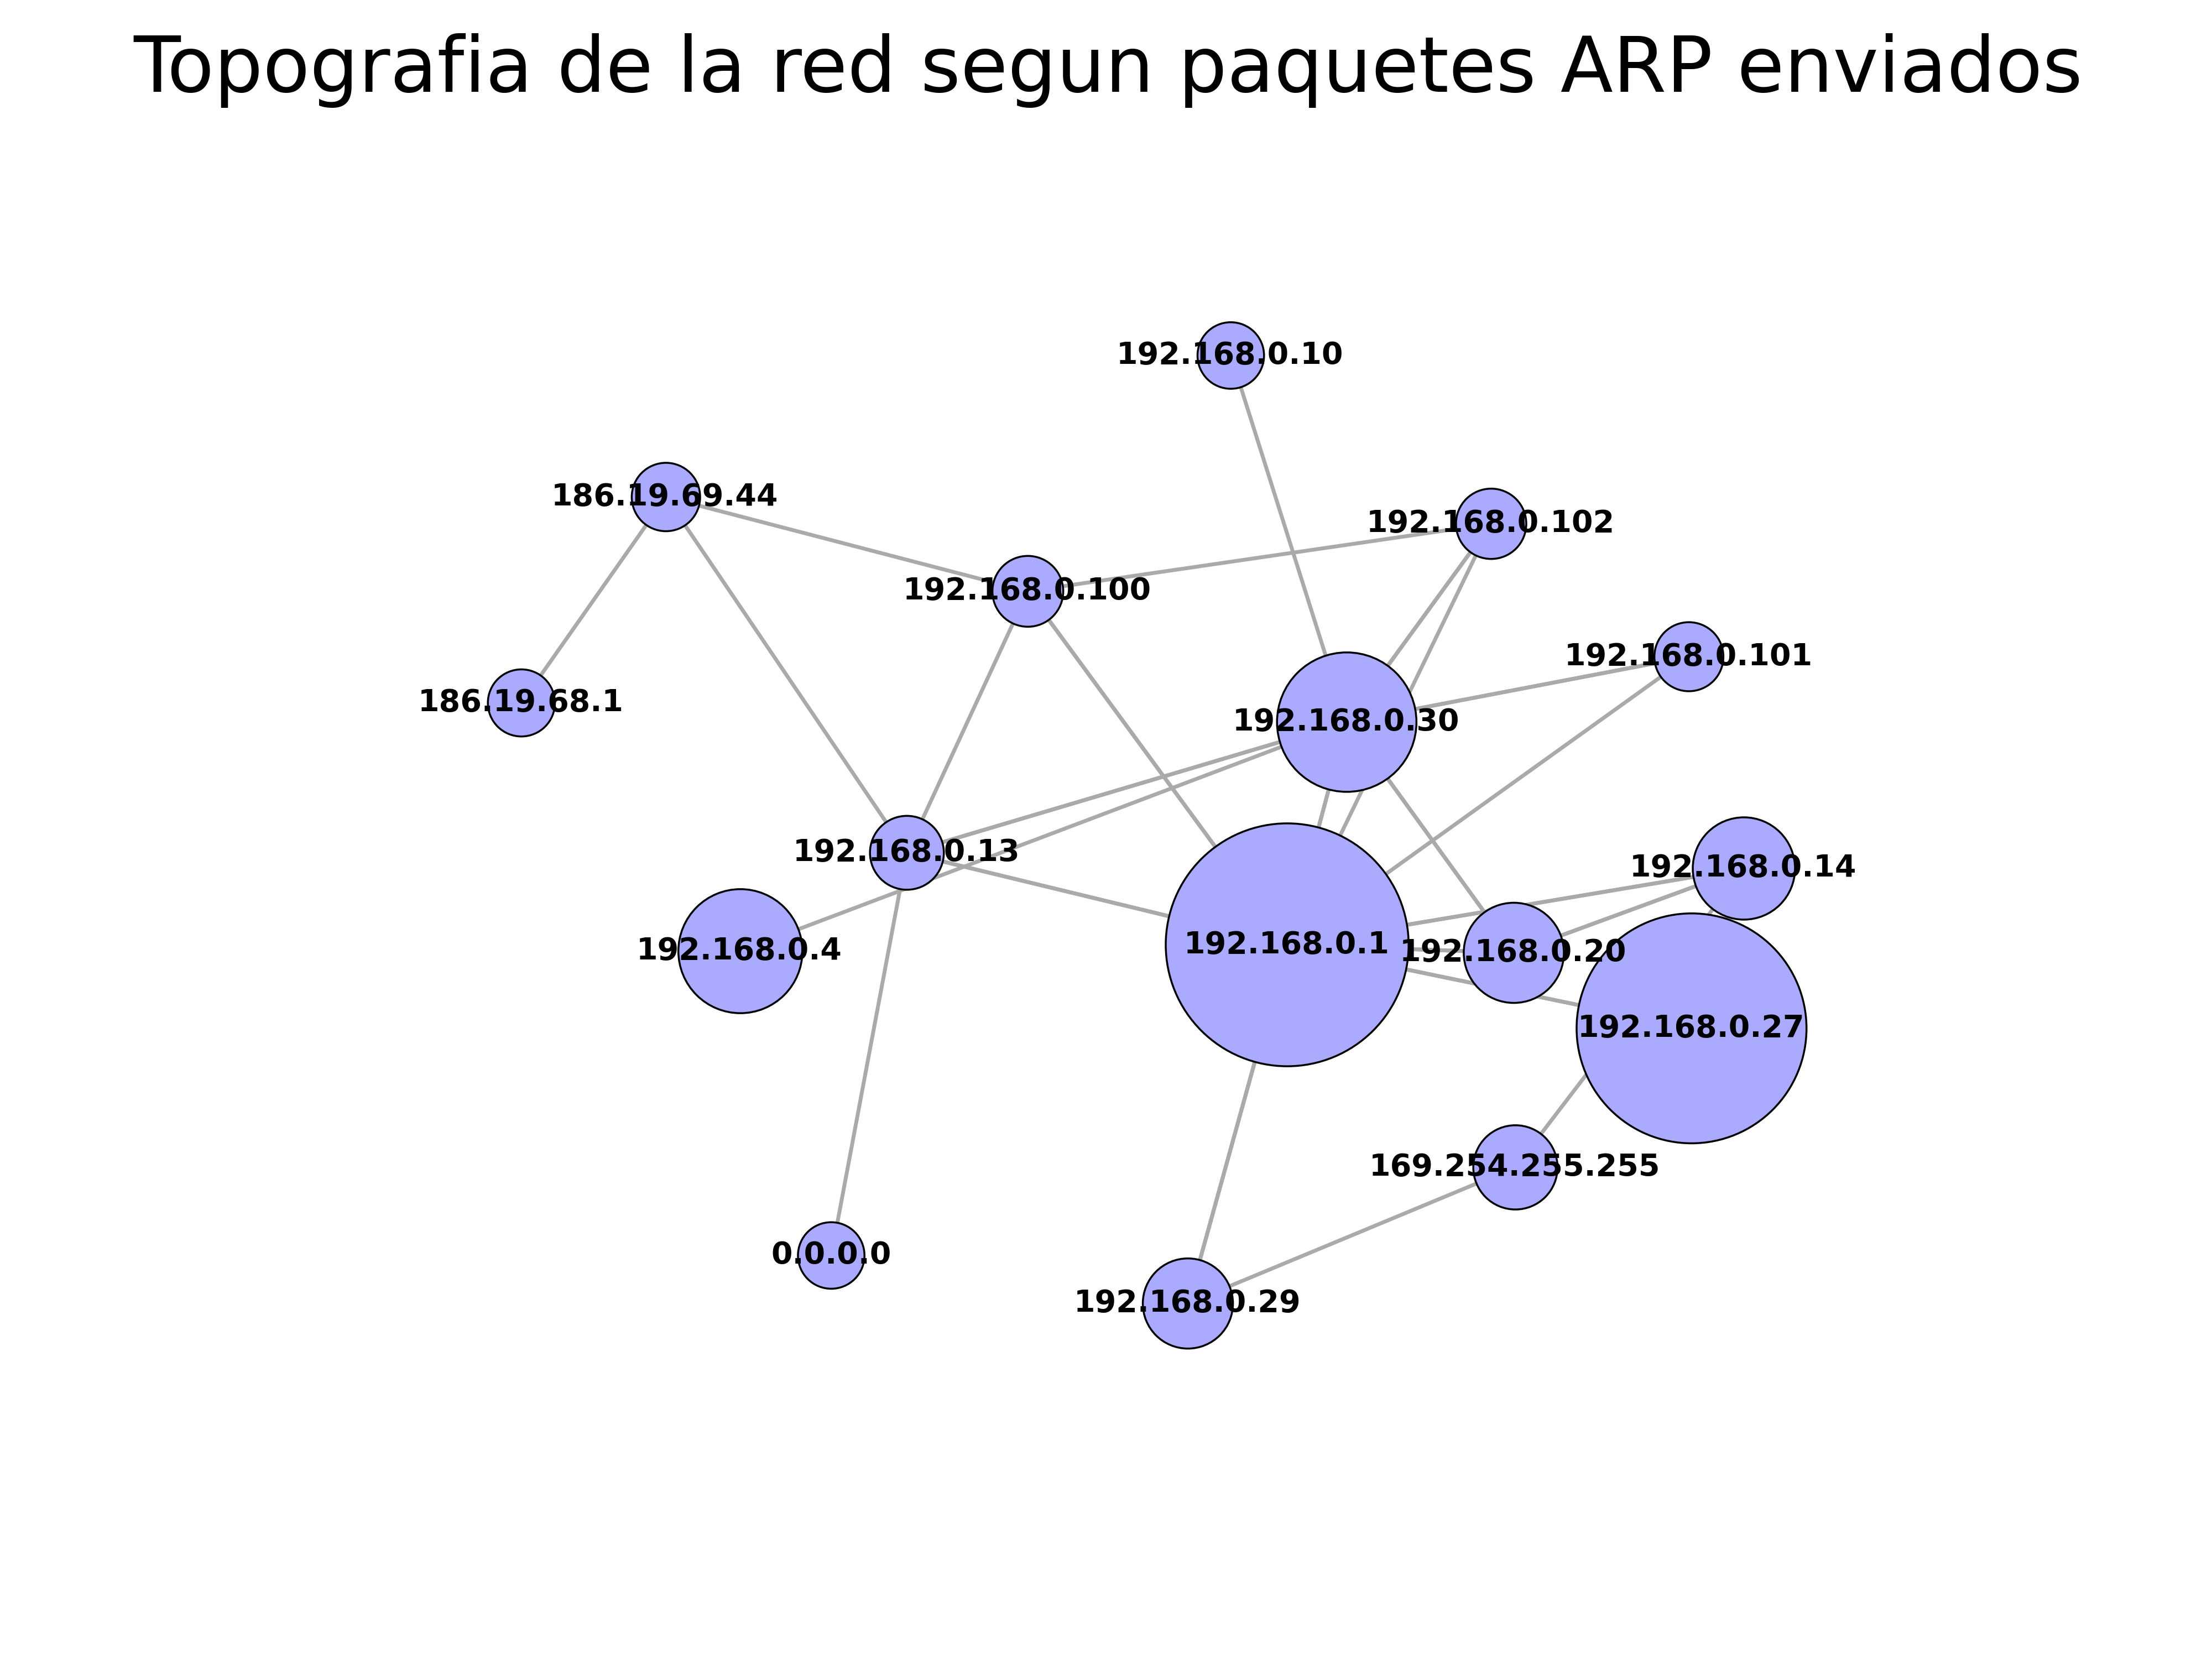
\includegraphics[width=0.7\textwidth]{graficos/red_domestica_network.png}
  \caption{Mi Figura}
  \label{fig:red_domestica_network}
\end{figure}

\FloatBarrier

\subsubsection{Histogramas (de IPs y protocolos)}

\begin{figure}[h!]
  \centering
   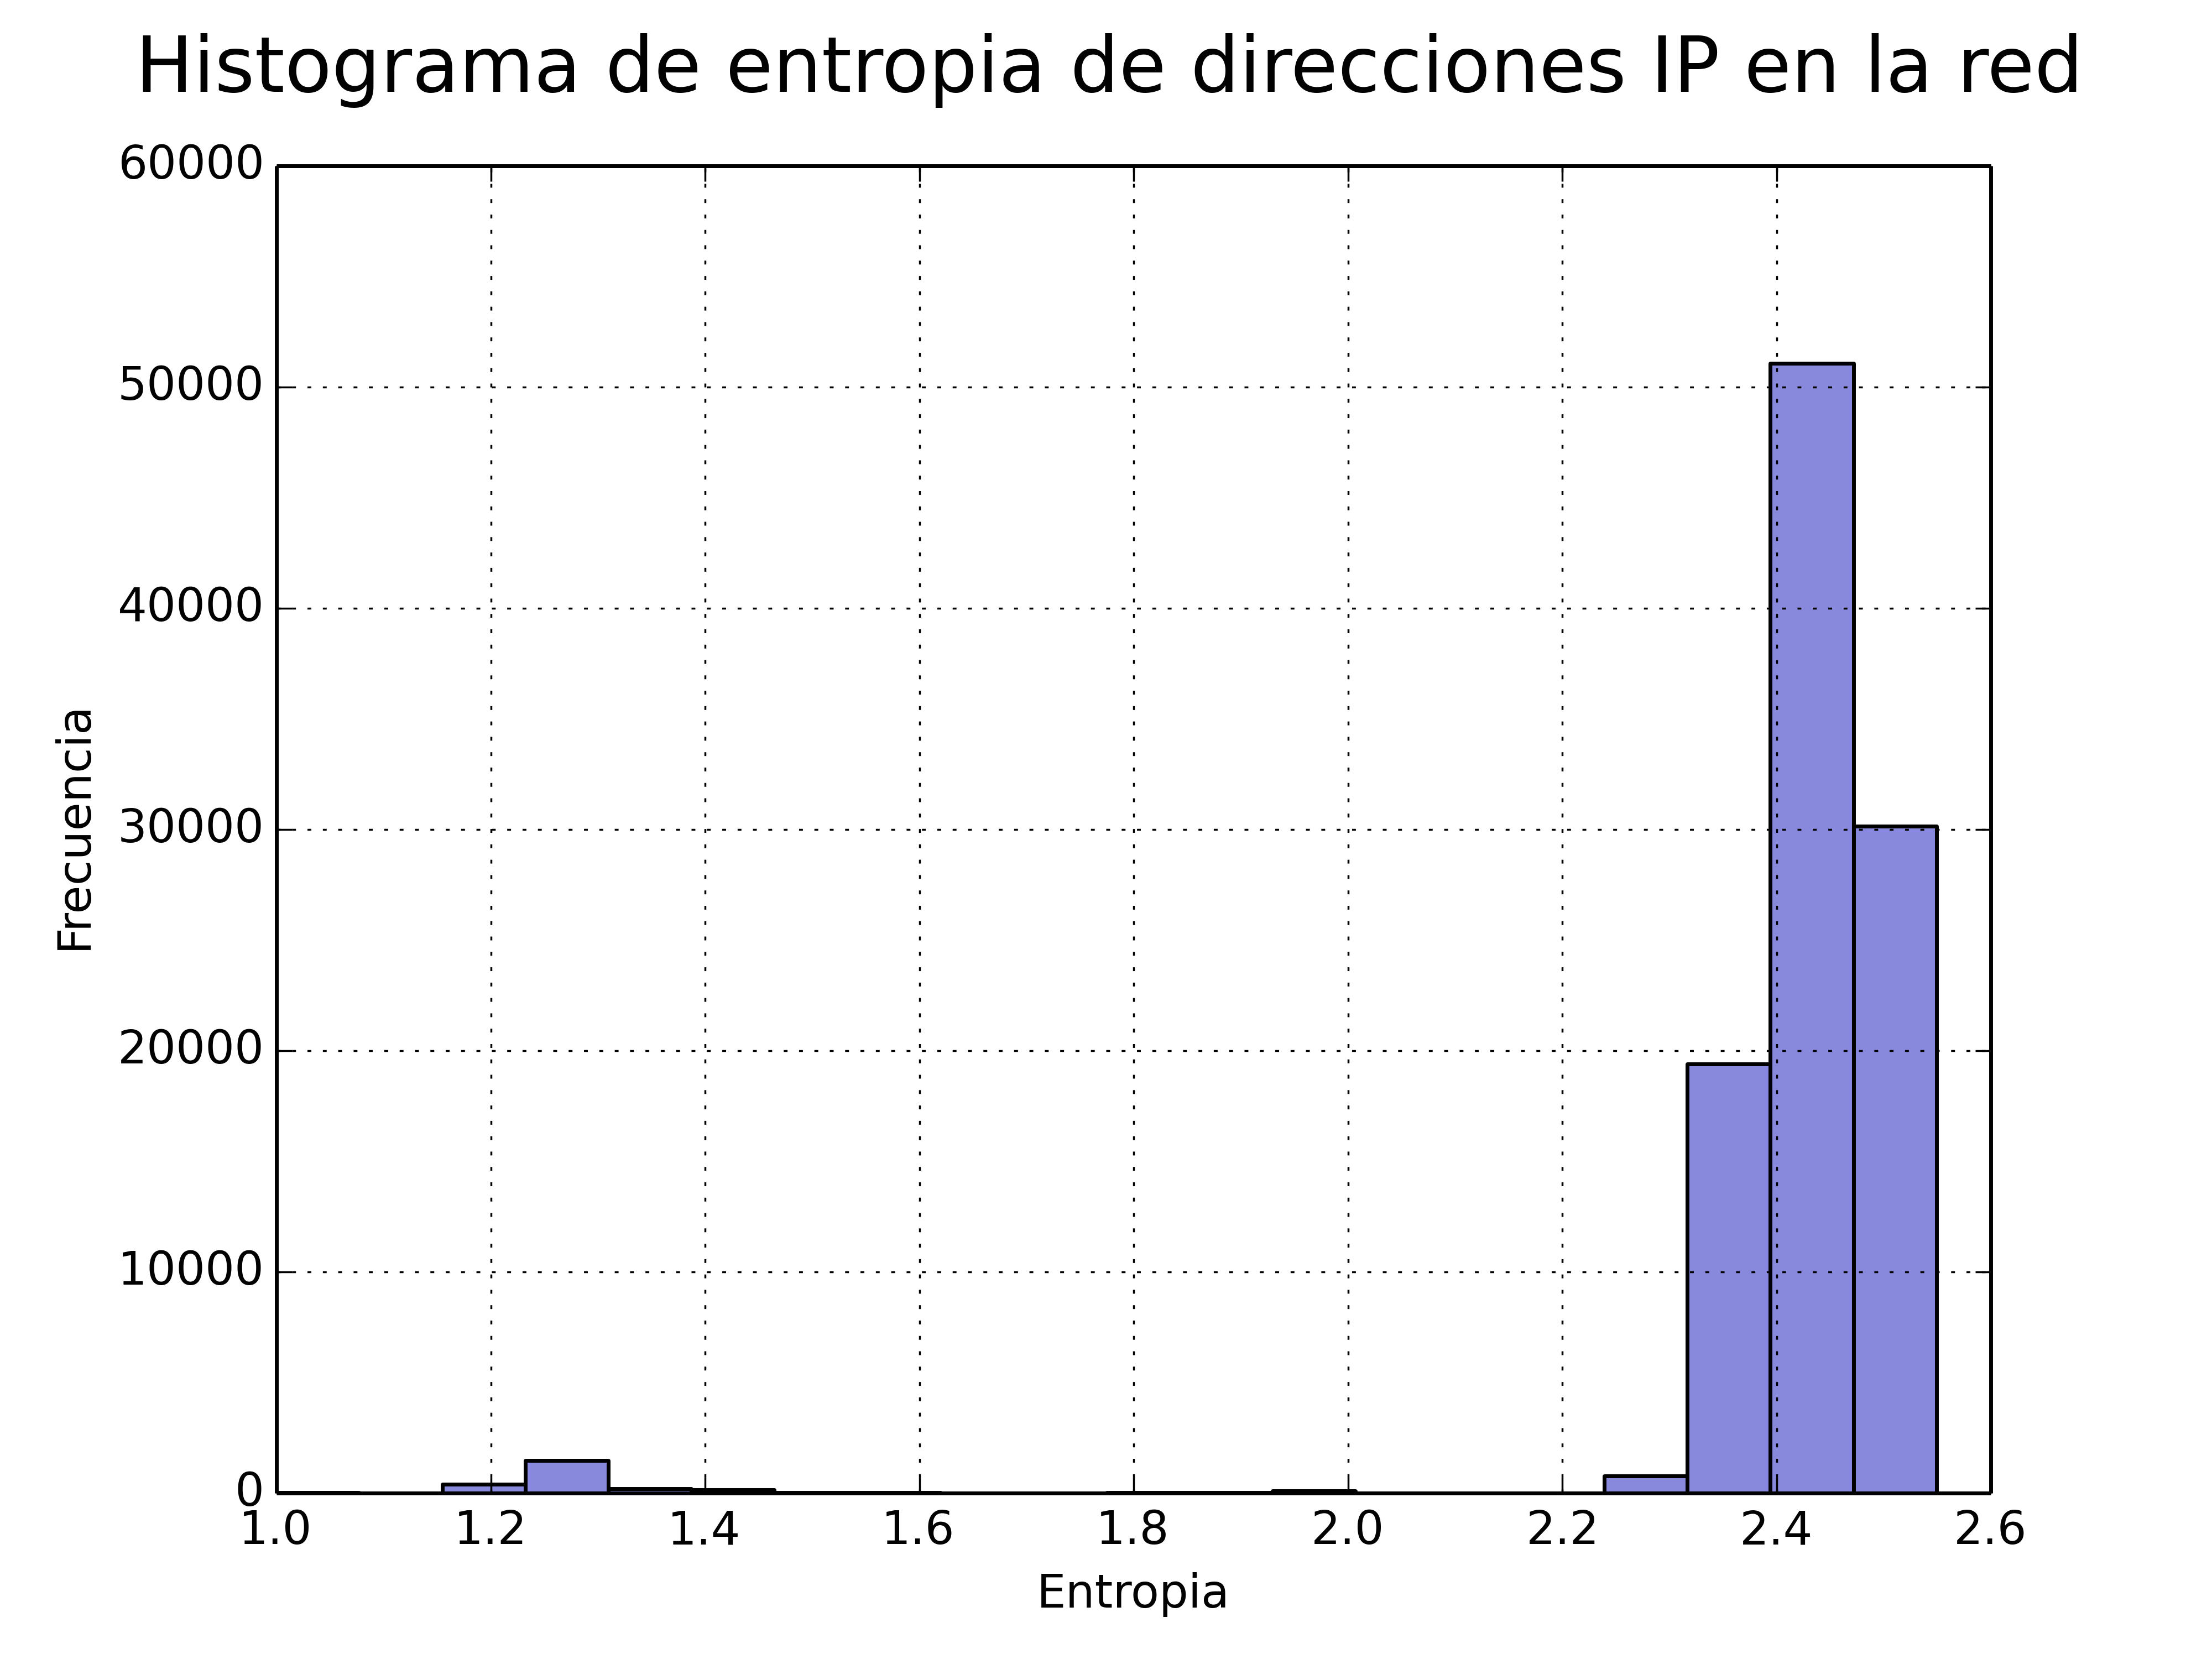
\includegraphics[width=0.7\textwidth]{graficos/red_domestica_hist_arp.png}
  \caption{Mi Figura}
  \label{fig:red_domestica_hist_arp}
\end{figure}

\begin{figure}[h!]
  \centering
   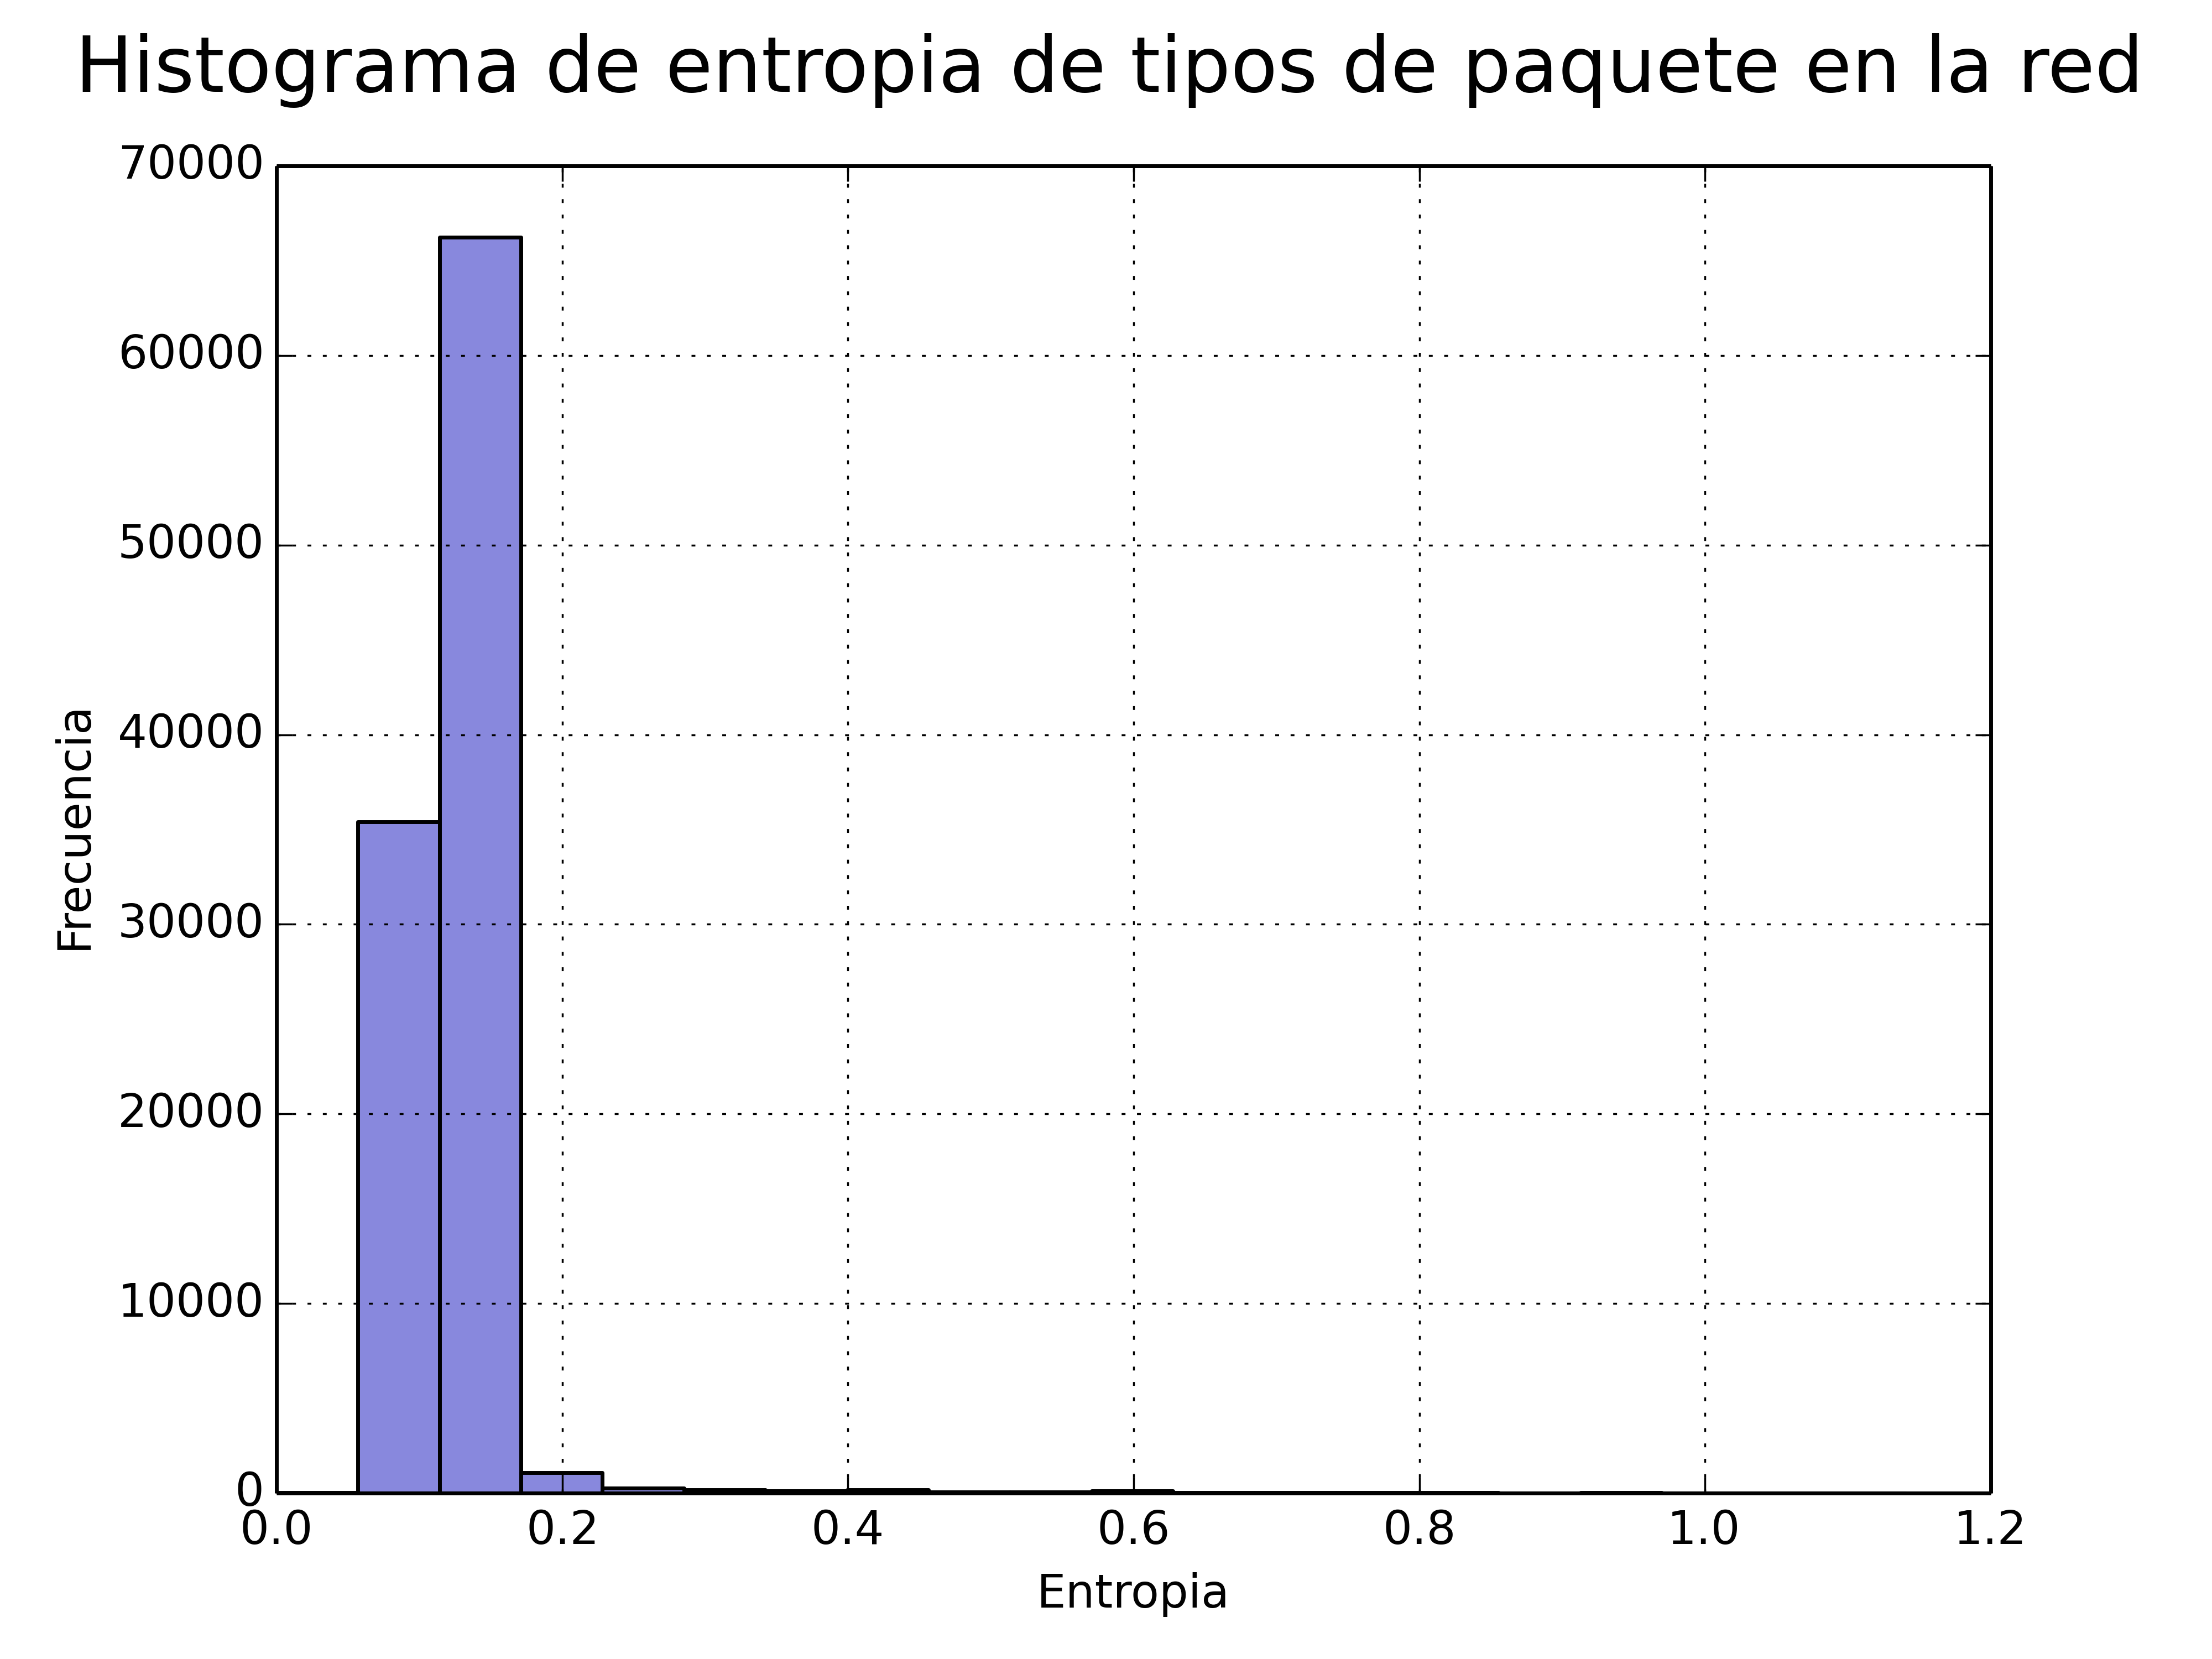
\includegraphics[width=0.7\textwidth]{graficos/red_domestica_hist_type.png}
  \caption{Mi Figura}
  \label{fig:red_domestica_hist_type}
\end{figure}

\FloatBarrier

\subsubsection{Paquetes capturados e información}

Los gráficos de torta, nos permiten ver la relación entre la cantidad de paquetes y la información que proveen cada nodo en la red. 
En los primeros 2 gráficos ~\ref{fig:red_domestica_pie_arp}. ~\ref{fig:red_domestica_pie_arp_information}. se toma como fuente las ips de la red.
Podemos notar que los nodos mencionados anteriormente son los mas frecuentes y por lo tanto los que menos información tienen.

En los siguientes 2 gráficos ~\ref{fig:red_domestica_pie_type}. ~\ref{fig:red_domestica_pie_type_information}. la fuente es la indicada en la cátedra. Vemos que el protocolo que mas se repite es el IP con un porcentaje muy superior al resto y aportando información casi nula. 

\begin{figure}[h!]
  \centering
   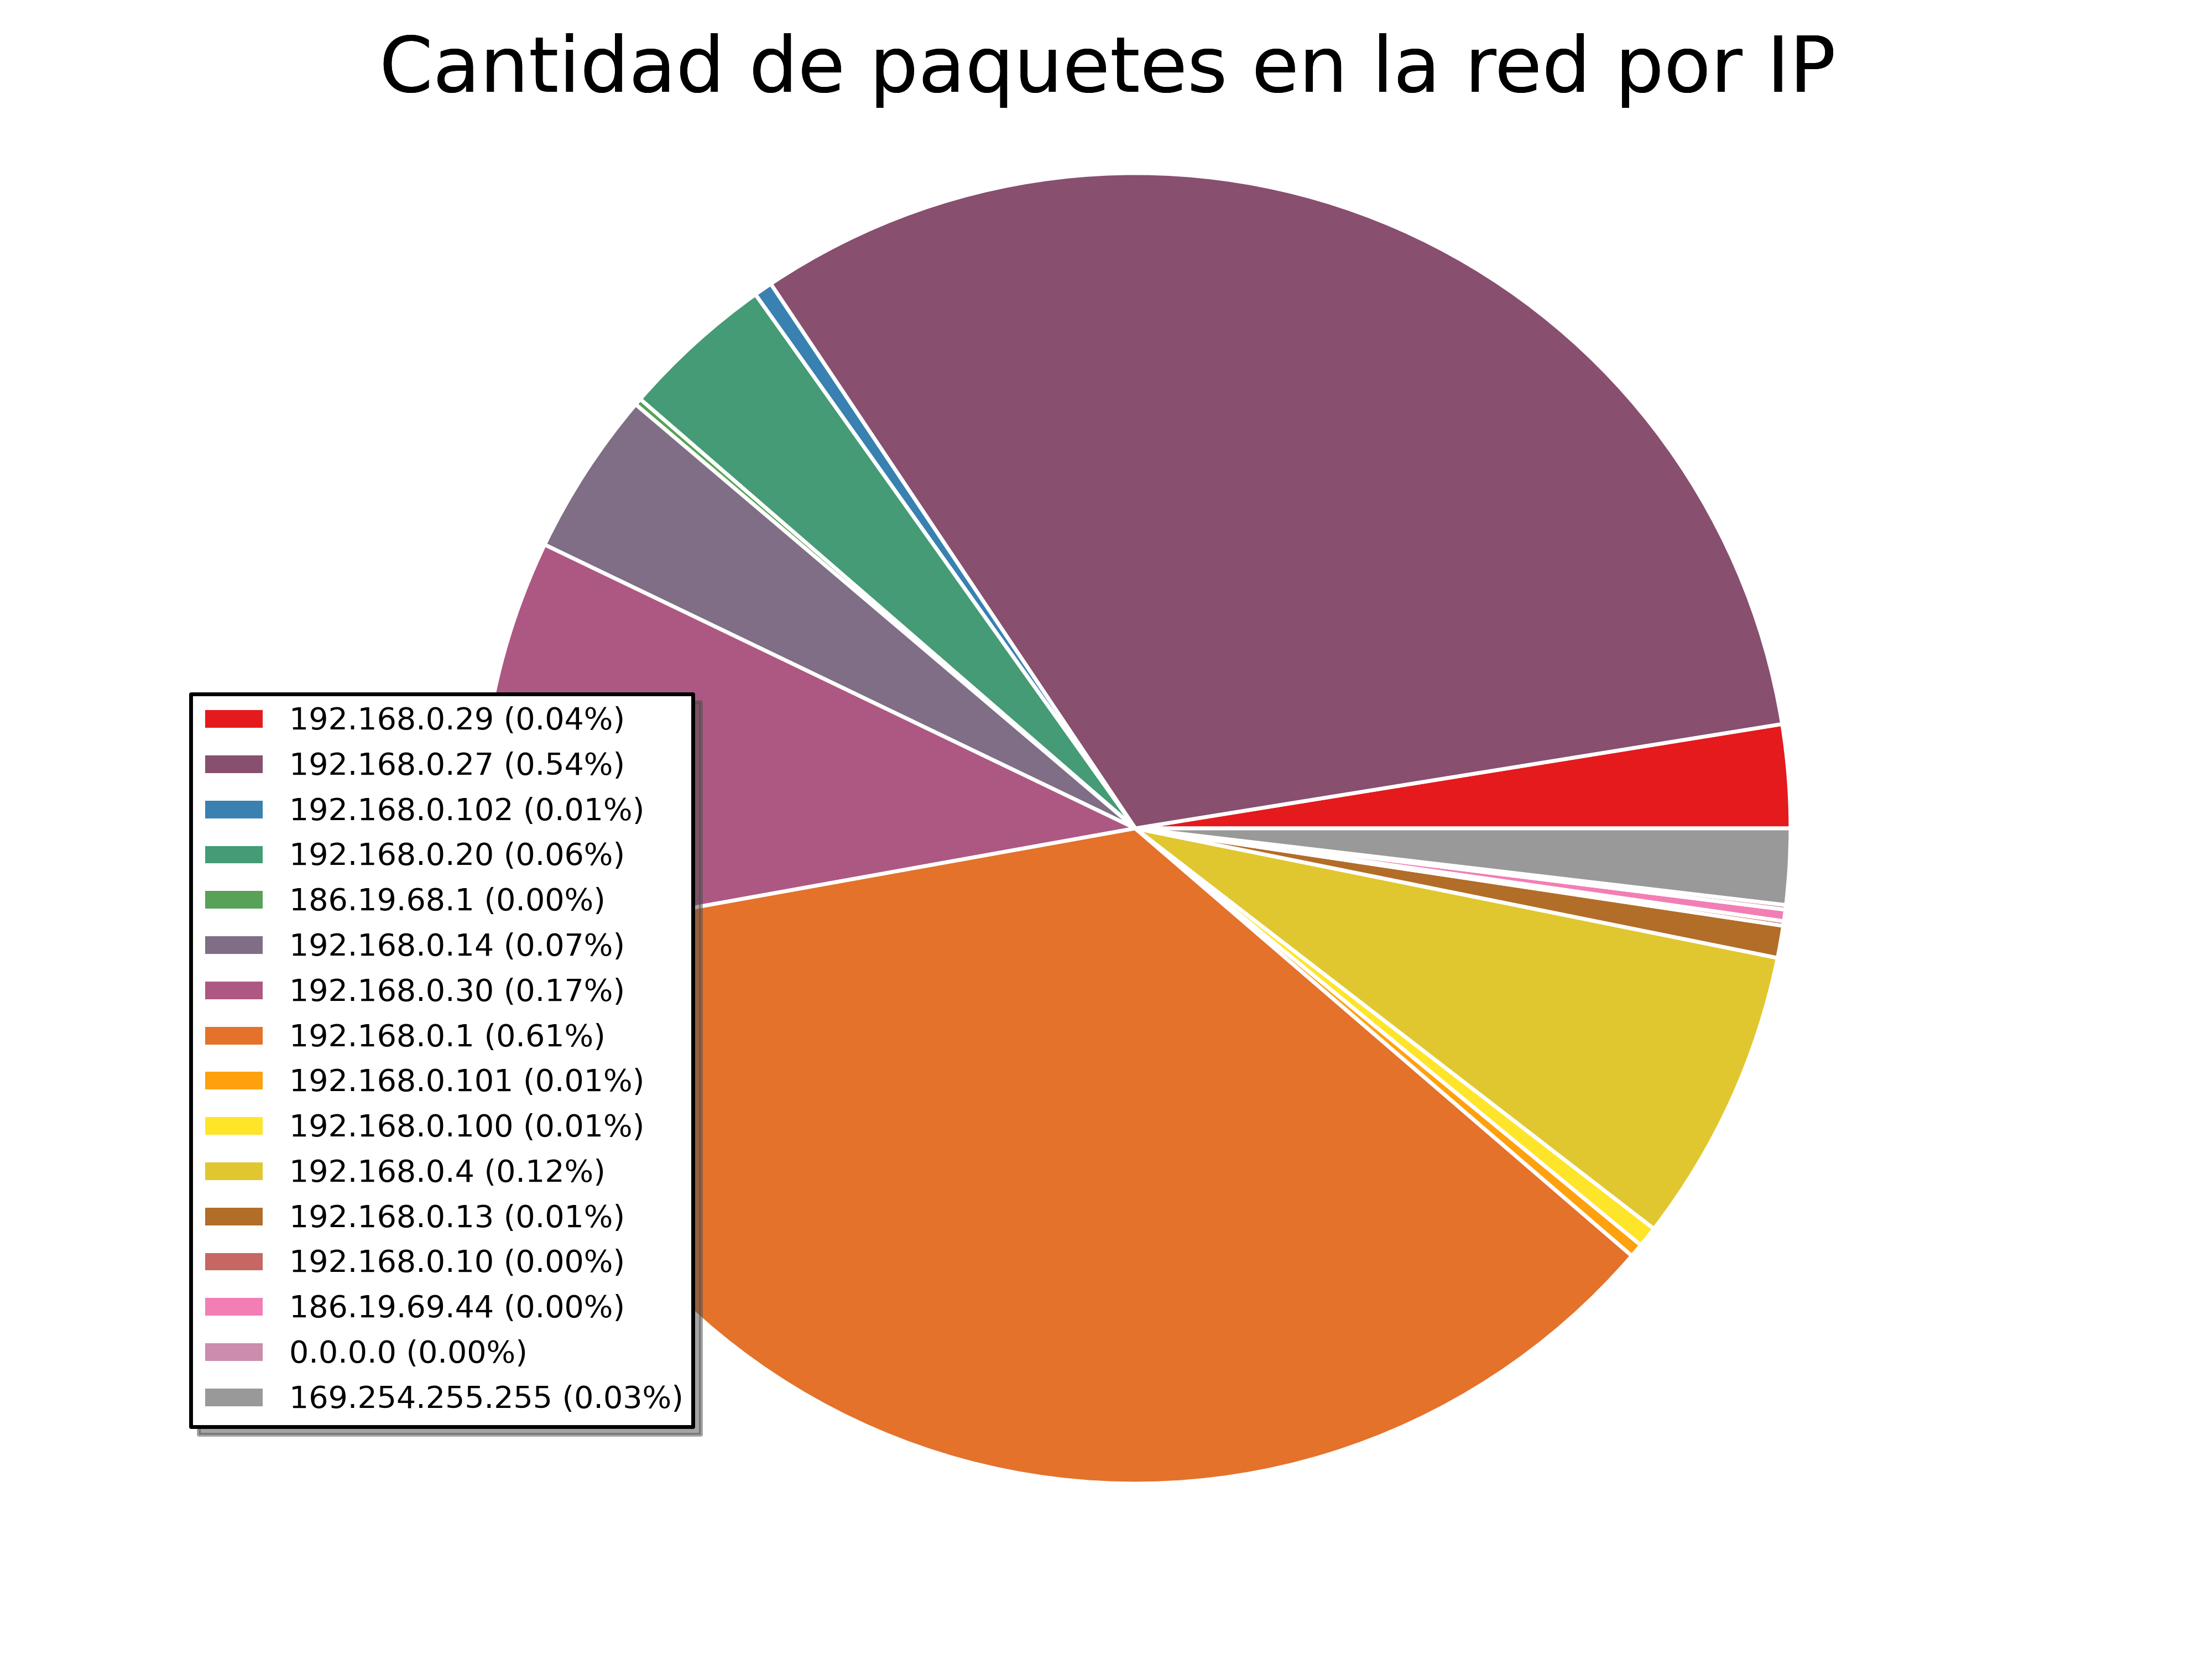
\includegraphics[width=0.7\textwidth]{graficos/red_domestica_pie_arp.png}
  \caption{Mi Figura}
  \label{fig:red_domestica_pie_arp}
\end{figure}

\begin{figure}[h!]
  \centering
   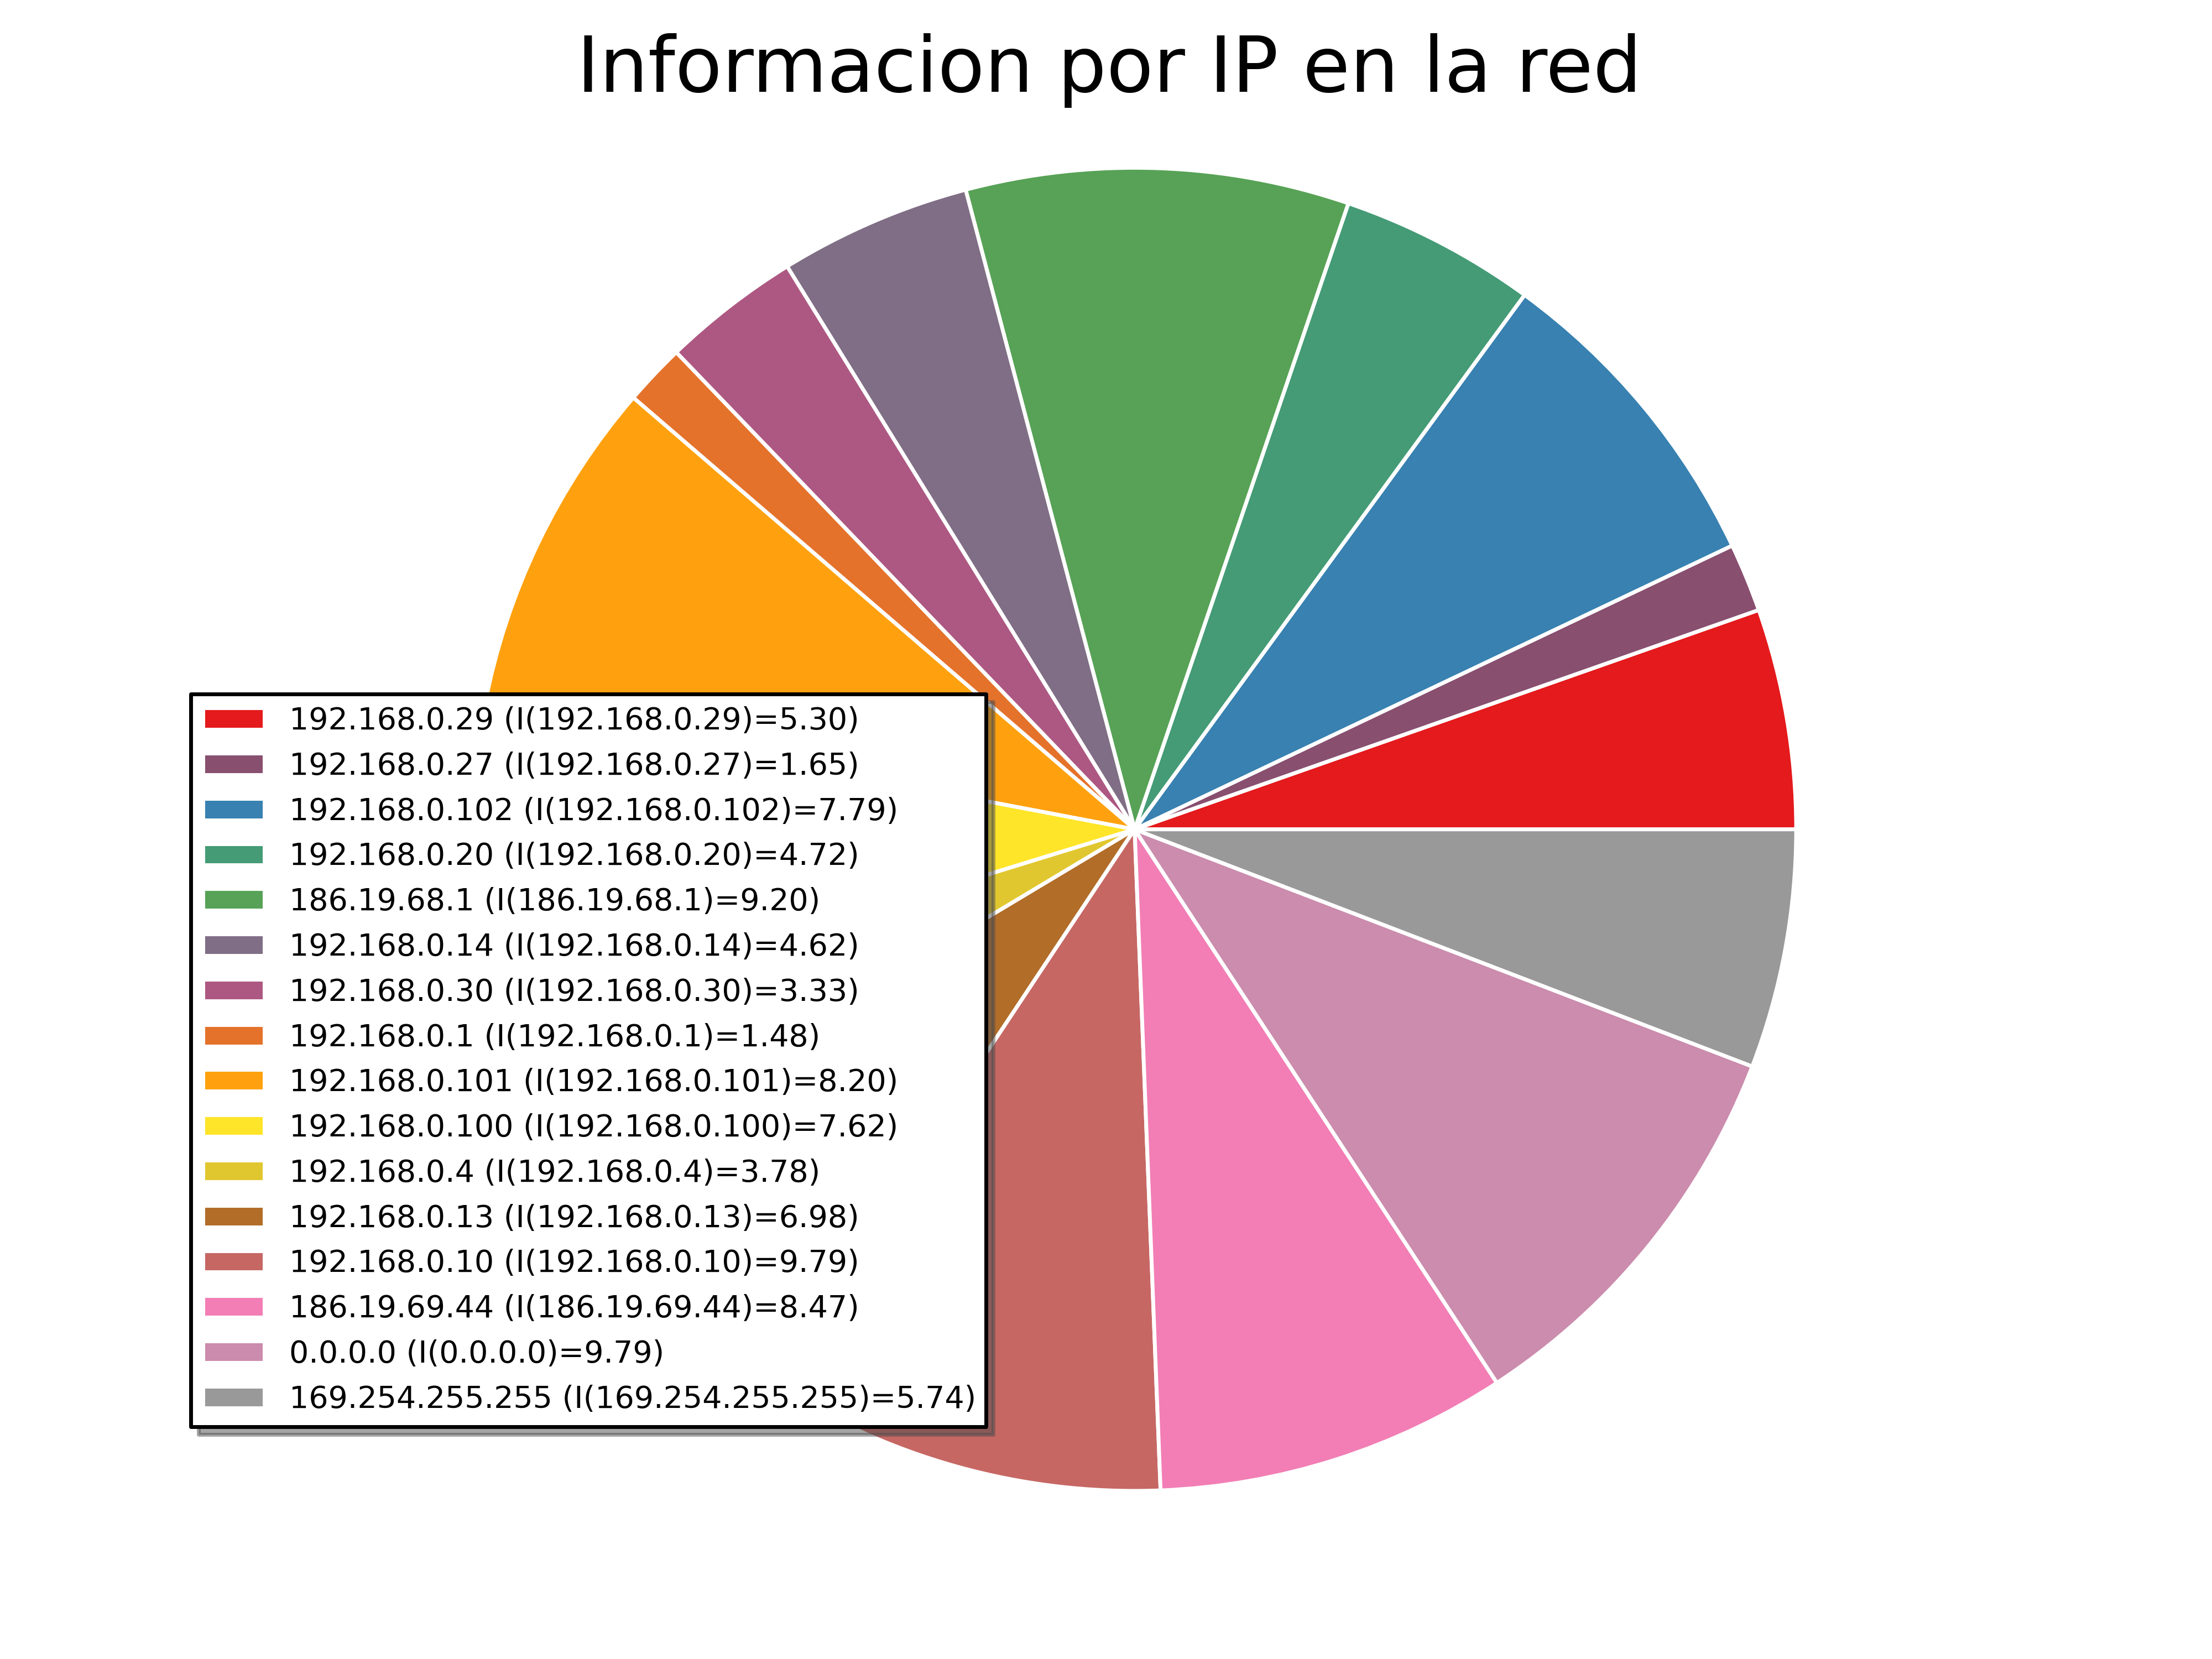
\includegraphics[width=0.7\textwidth]{graficos/red_domestica_pie_arp_information.png}
  \caption{Mi Figura}
  \label{fig:red_domestica_pie_arp_information}
\end{figure}

\begin{figure}[h!]
  \centering
   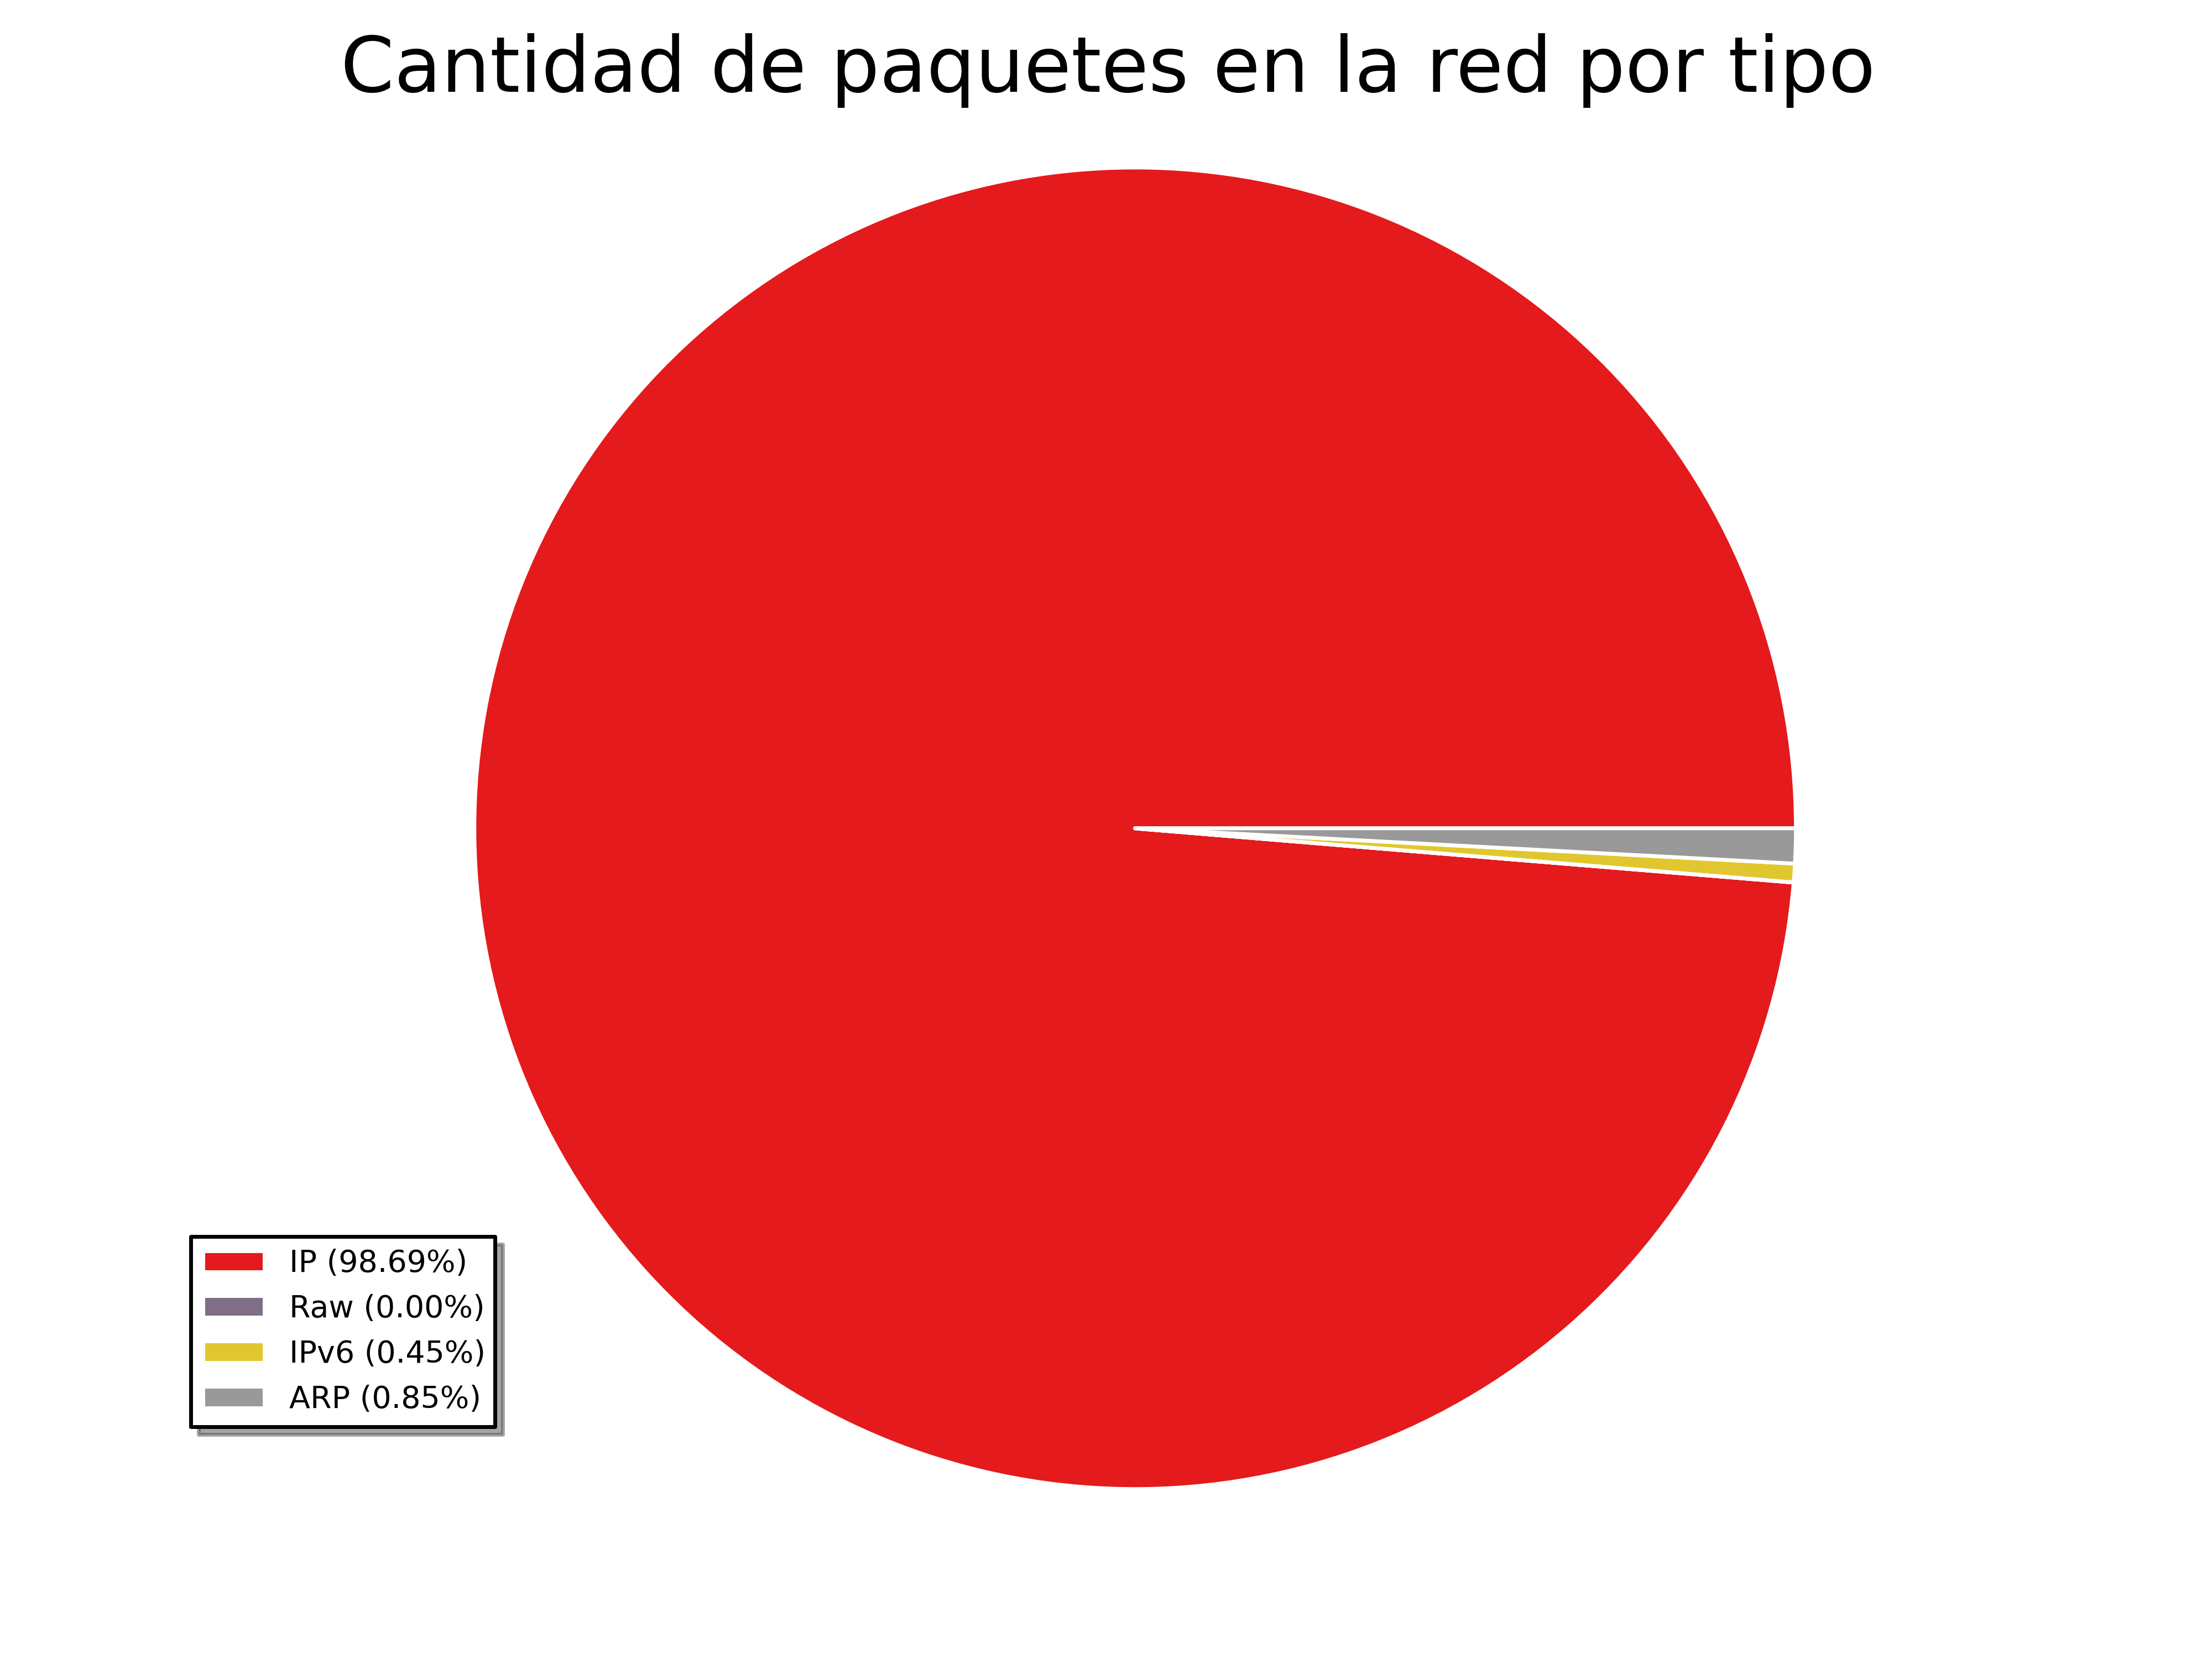
\includegraphics[width=0.7\textwidth]{graficos/red_domestica_pie_type.png}
  \caption{Mi Figura}
  \label{fig:red_domestica_pie_type}
\end{figure}

\begin{figure}[h!]
  \centering
   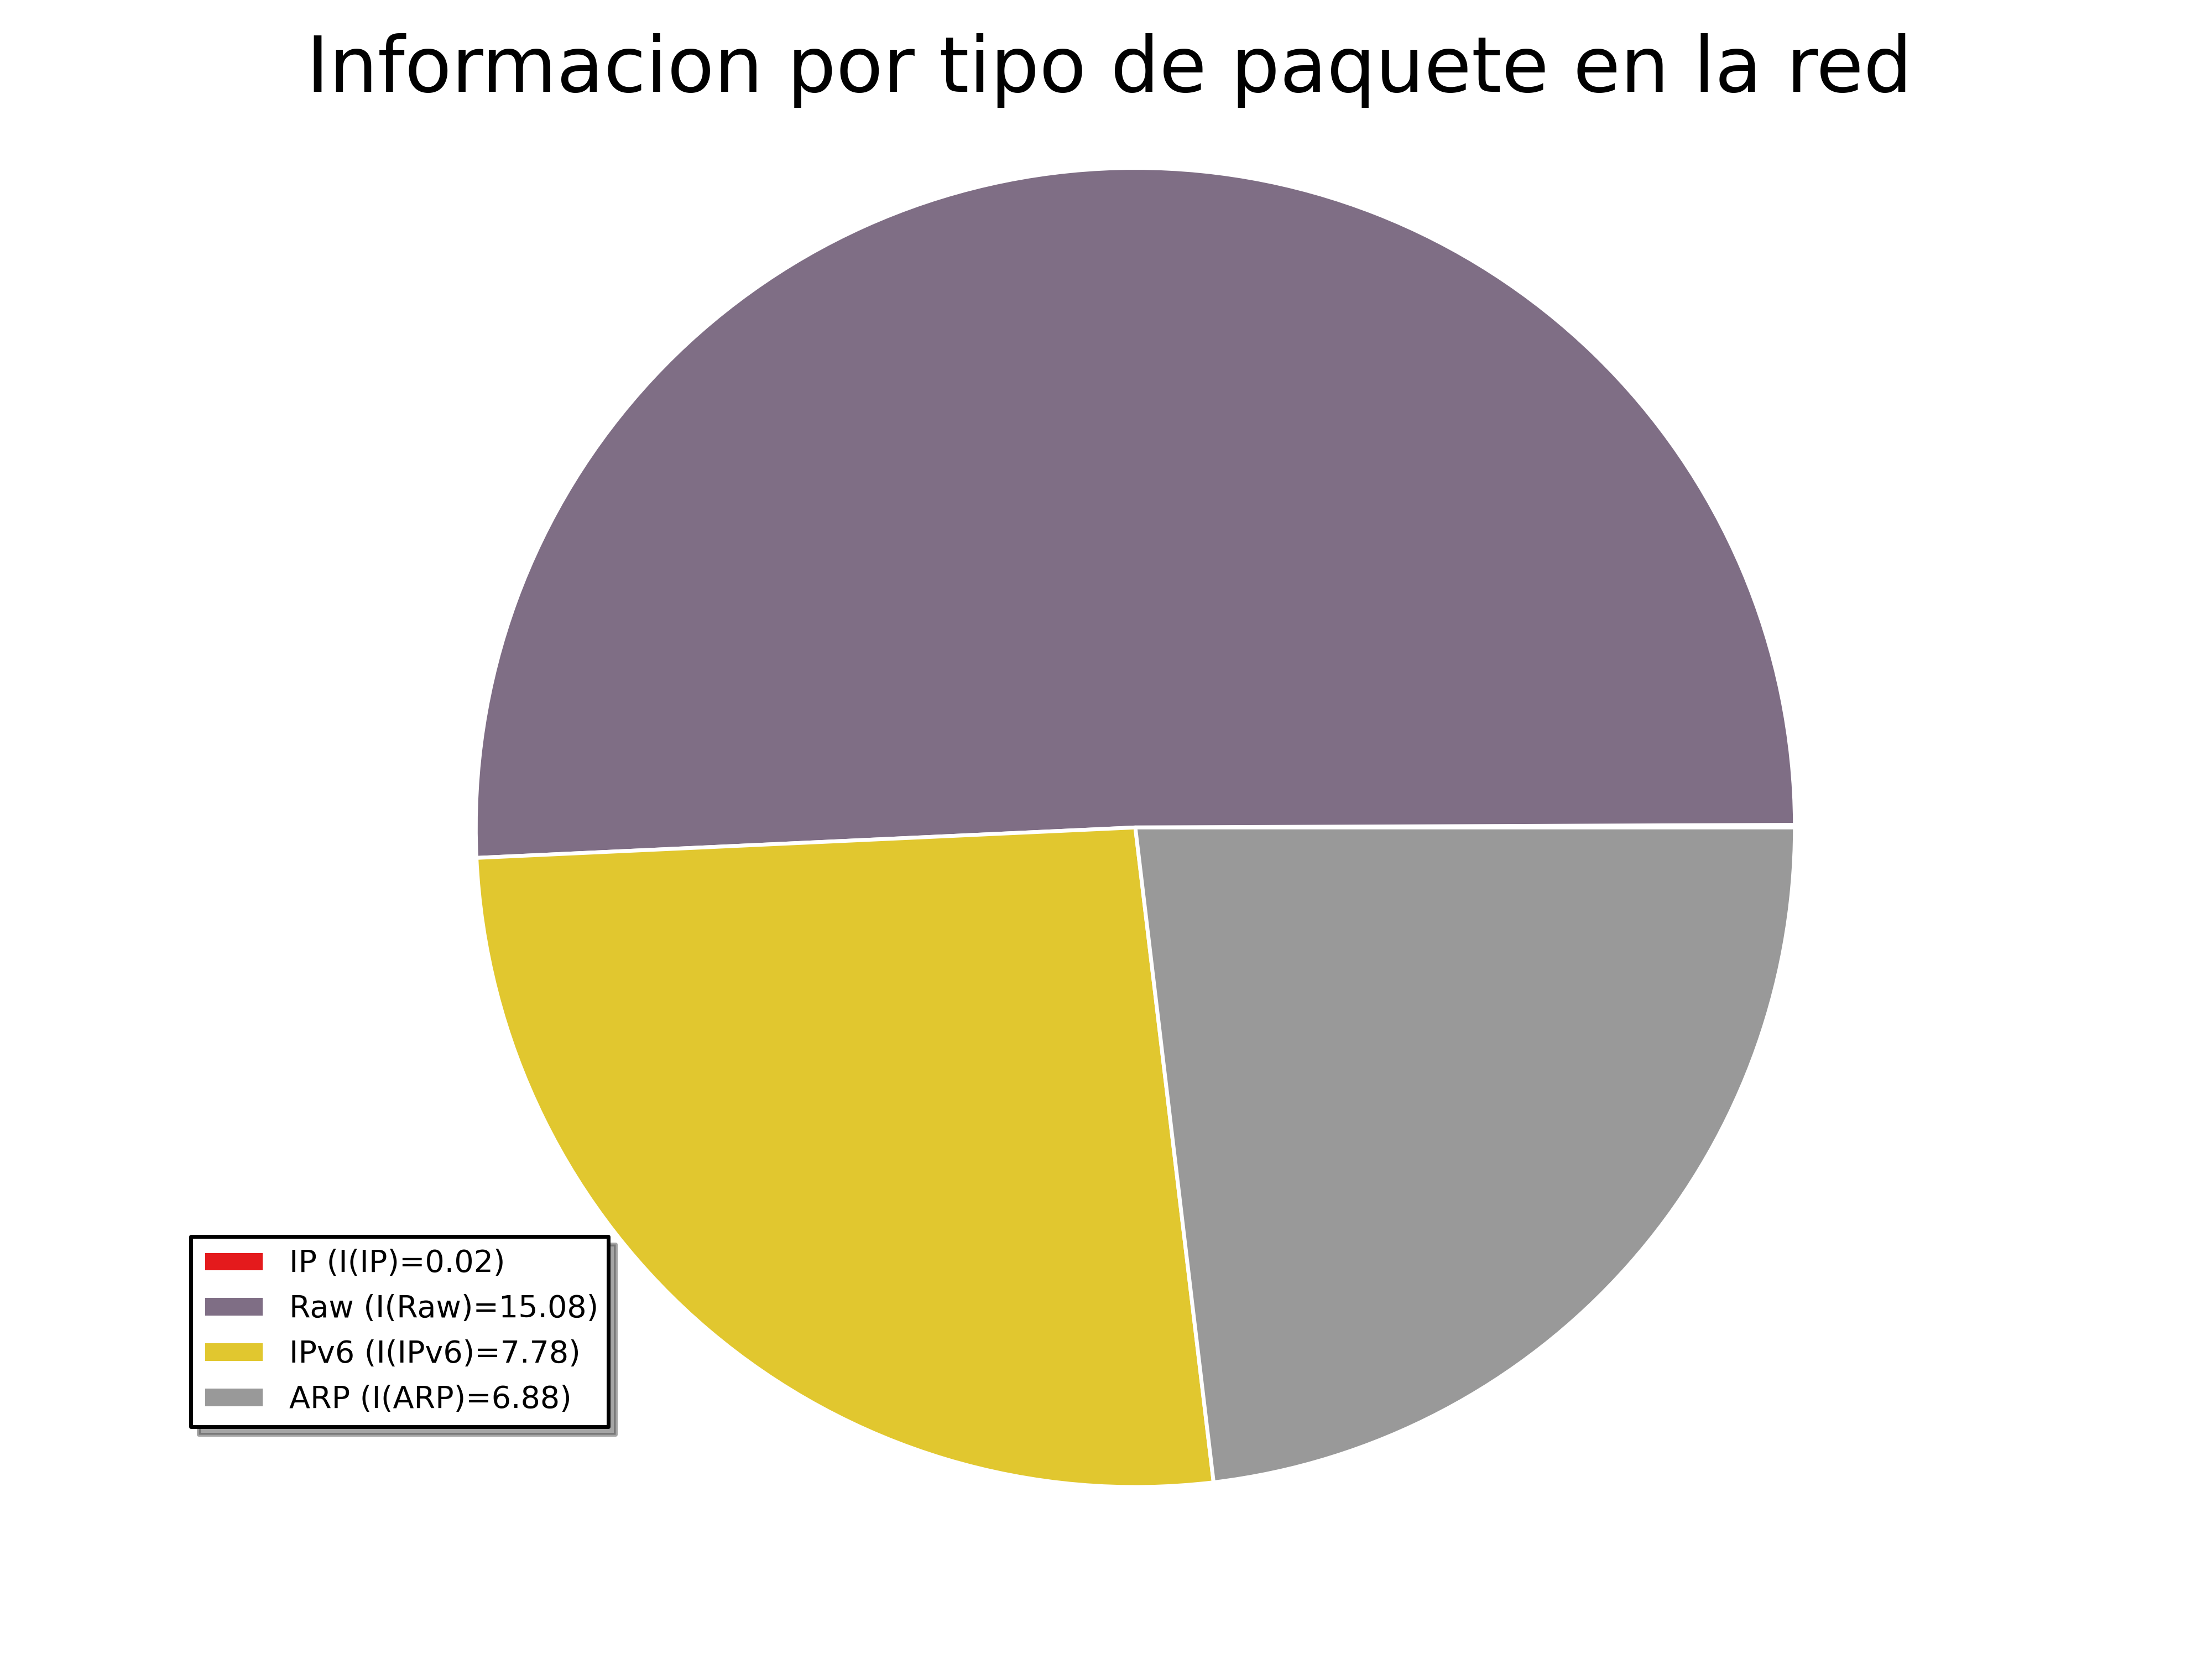
\includegraphics[width=0.7\textwidth]{graficos/red_domestica_pie_type_information.png}
  \caption{Mi Figura}
  \label{fig:red_domestica_pie_type_information}
\end{figure}